%#!platex ./report.tex

%
% $B2r@O9`L\$N@bL@$r(BMethod$B$KF~$l$F$*$/!"(BUpper Dend, Lower Dend$B$NDj5A$r$7$F$*$-$?$$(B
%

%
% $B$=$l$>$l$N%Q%?!<%s$G$NH/2P$NMM;R$b$$$l$F$*$$$?$[$&$,$$$$(B -> $B?^$,BgNL$K$J$k(B
%

% 
% $B%3%s%@%/%?%s%9NL$N8!Dj$ON>B&$G$O$J$/!"!V8:$C$?$+!W$I$&$+$r$_$l$P$$$$$N$G$O!)(B
%


\chapter{$B7k2L(B}
 \section{Passive$B$N7k2L(B}
   \subsection{$B@h9T8&5f<jK!(B\cite{torben2009systematic}$B$H$NHf3S(B}
     $BK\8&5f<jK!$H@h9T8&5f$GMQ$$$i$l$F$$$?8DBNI>2A;XI8$H$NHf3S$r0J2<$N(B
     $B?^(B\ref{Tsuishi_Rerative1}, $B?^(B\ref{Tsuishi_Rerative2}$B$K<($9(B. 
     $B?^Cf$N(BTorben et al.$B$O@h9T8&5f<jK!$rMQ$$$?7k2L$G$"$j(B, Rerative$B$OK\8&5f$rMQ$$$?7k2L$G$"$k(B.

%subfigure $B$rF~$l$k$H$-$K2~9T$9$k$H!"<B:]$NJ8>O$G$b2~9T$,H?1G$5$l!"2#$KJB$P$J$/$J$k$k$N$GCm0U(B
     \begin{figure}[H]
       \begin{subfigure}{0.5\columnwidth}
         \centering
         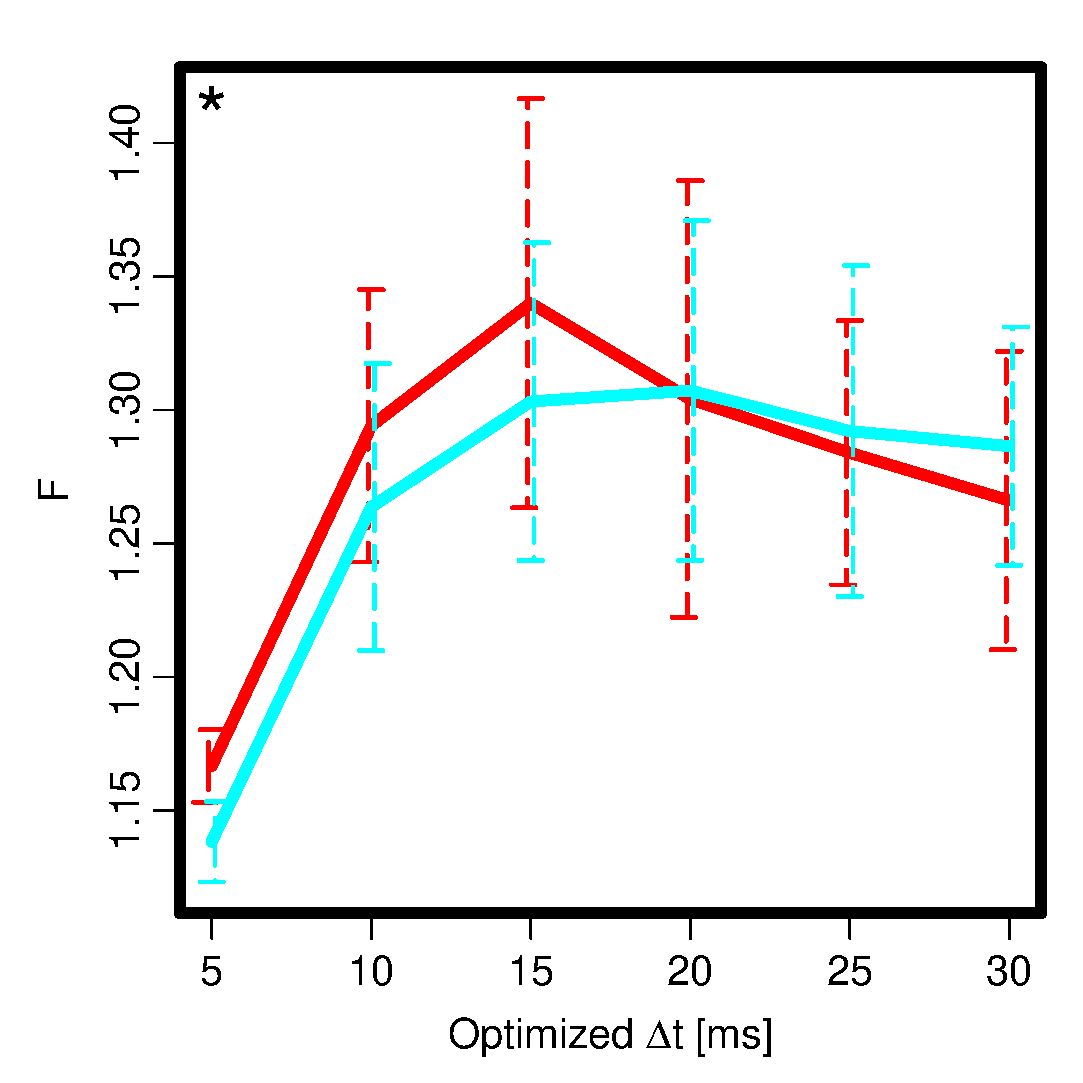
\includegraphics[width=0.8\columnwidth]{./Images_Result/Tsuishi_Rerative_F.eps} 
         \caption{F}
         \label{Tsuishi_Rerative_F}
       \end{subfigure}
       \begin{subfigure}{0.5\columnwidth}
         \centering
         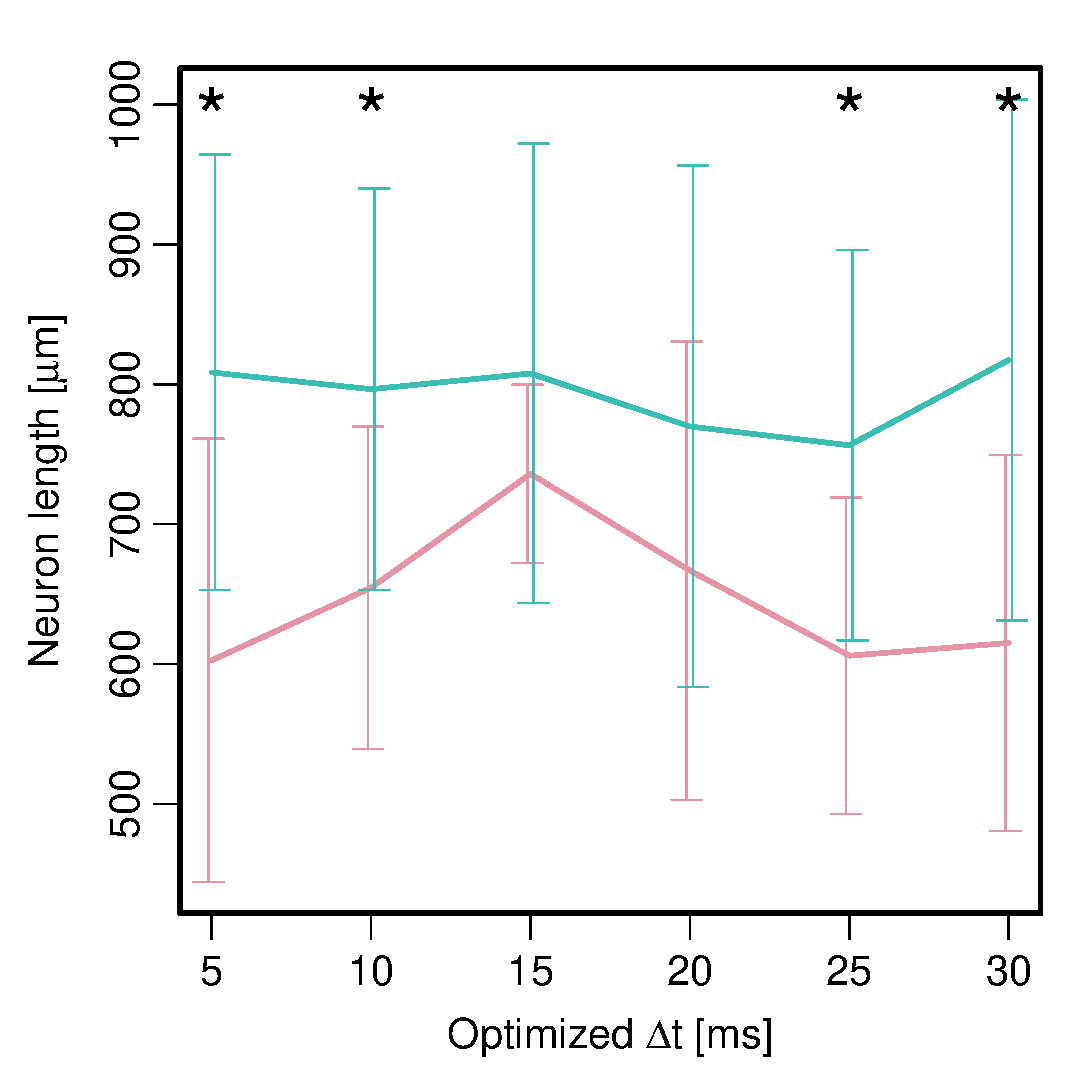
\includegraphics[width=0.8\columnwidth]{./Images_Result/Tsuishi_Rerative_TREE_length.eps} 
         \caption{$BD9$5(B}
         \label{Tsuishi_Rerative_length}
       \end{subfigure}

       \begin{subfigure}{0.5\columnwidth}
         \centering
         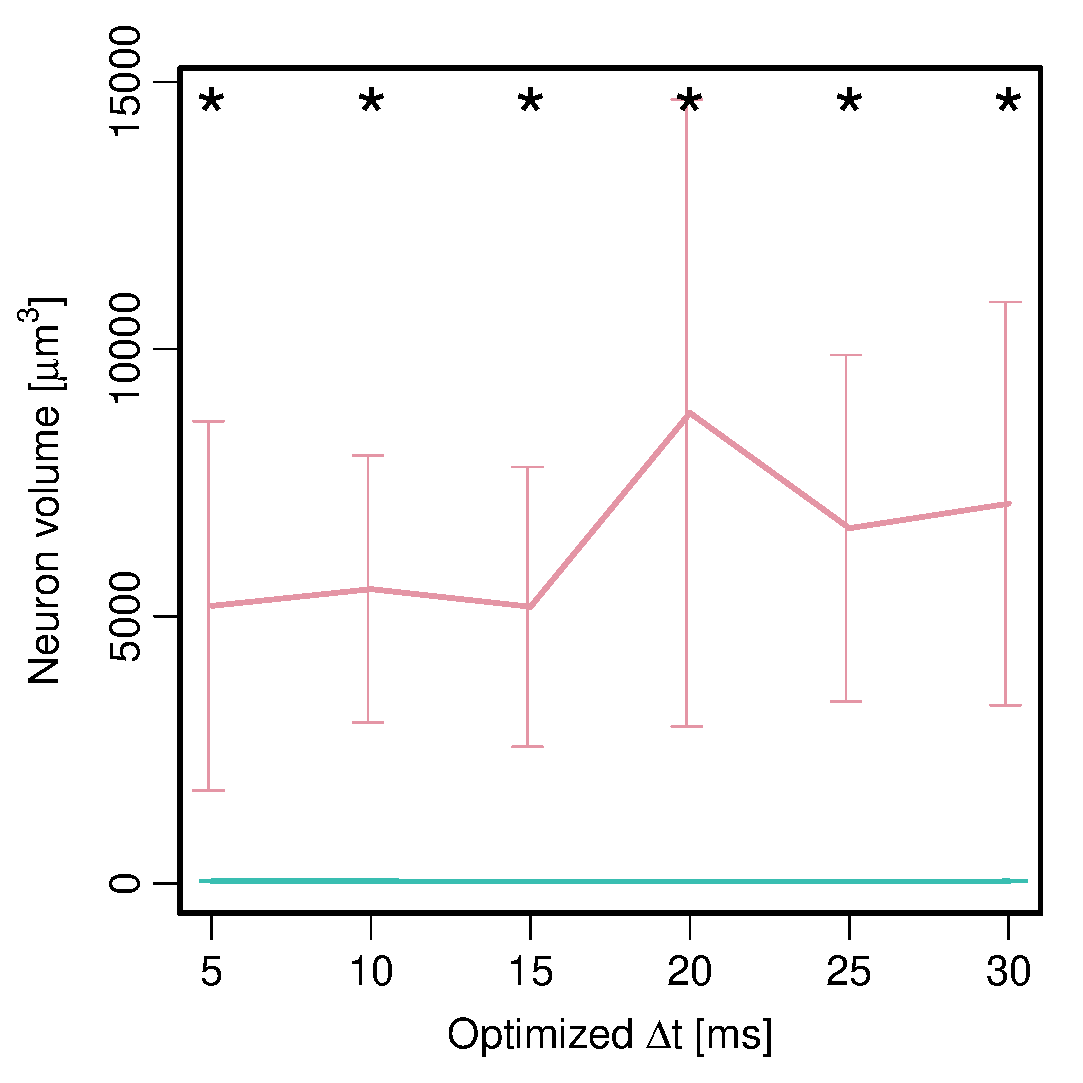
\includegraphics[width=0.8\columnwidth]{./Images_Result/Tsuishi_Rerative_TREE_volume.eps} 
         \caption{$BBN@Q(B}
         \label{Tsuishi_Rerative_volume}
       \end{subfigure}
       \begin{subfigure}{0.5\columnwidth}
         \centering
         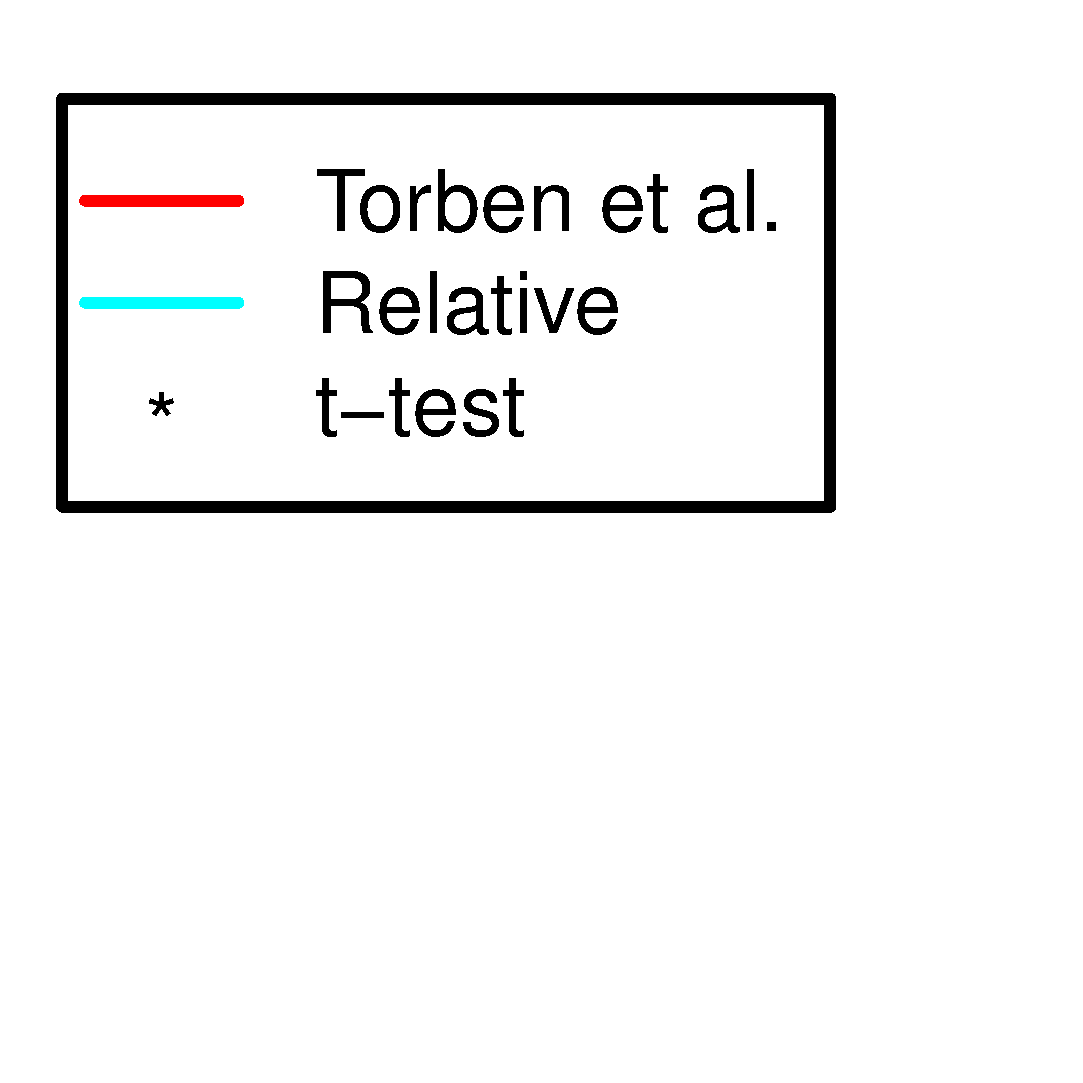
\includegraphics[width=0.8\columnwidth]{./Images_Result/Tsuishi_Rerative_legend.eps} 
       \end{subfigure}

       \caption{$B@h9T8&5f<jK!$H$NHf3S(B1}
       \label{Tsuishi_Rerative1}
     \end{figure}

     \begin{figure}[H]
       \begin{subfigure}{0.5\columnwidth}
         \centering
         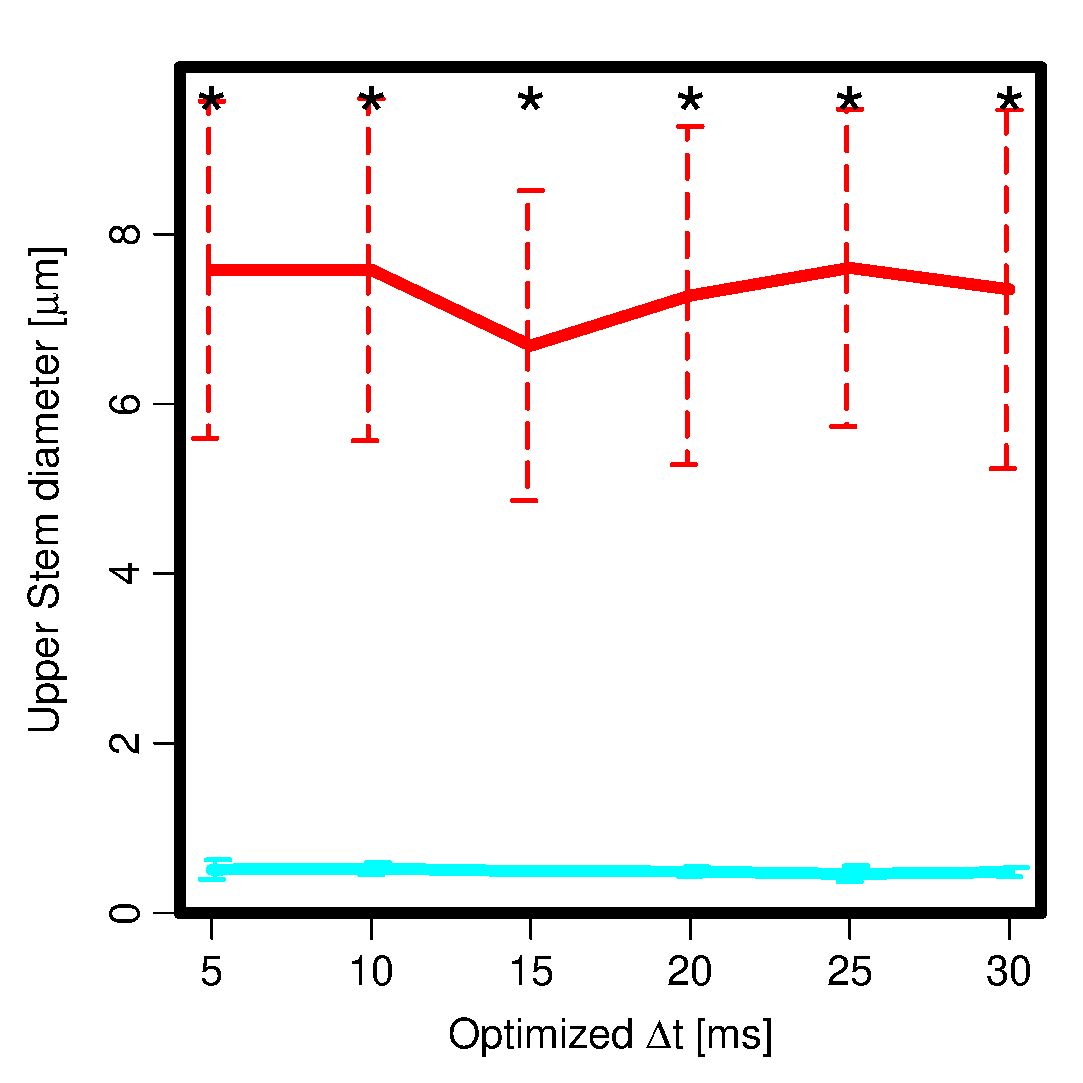
\includegraphics[width=0.8\columnwidth]{./Images_Result/Tsuishi_Rerative_Upper_Diam.eps} 
         \caption{Upper Dendrite$B$ND>7B(B}
         \label{Tsuishi_Rerative_Upper_Diam}
       \end{subfigure}
       \begin{subfigure}{0.5\columnwidth}
         \centering
         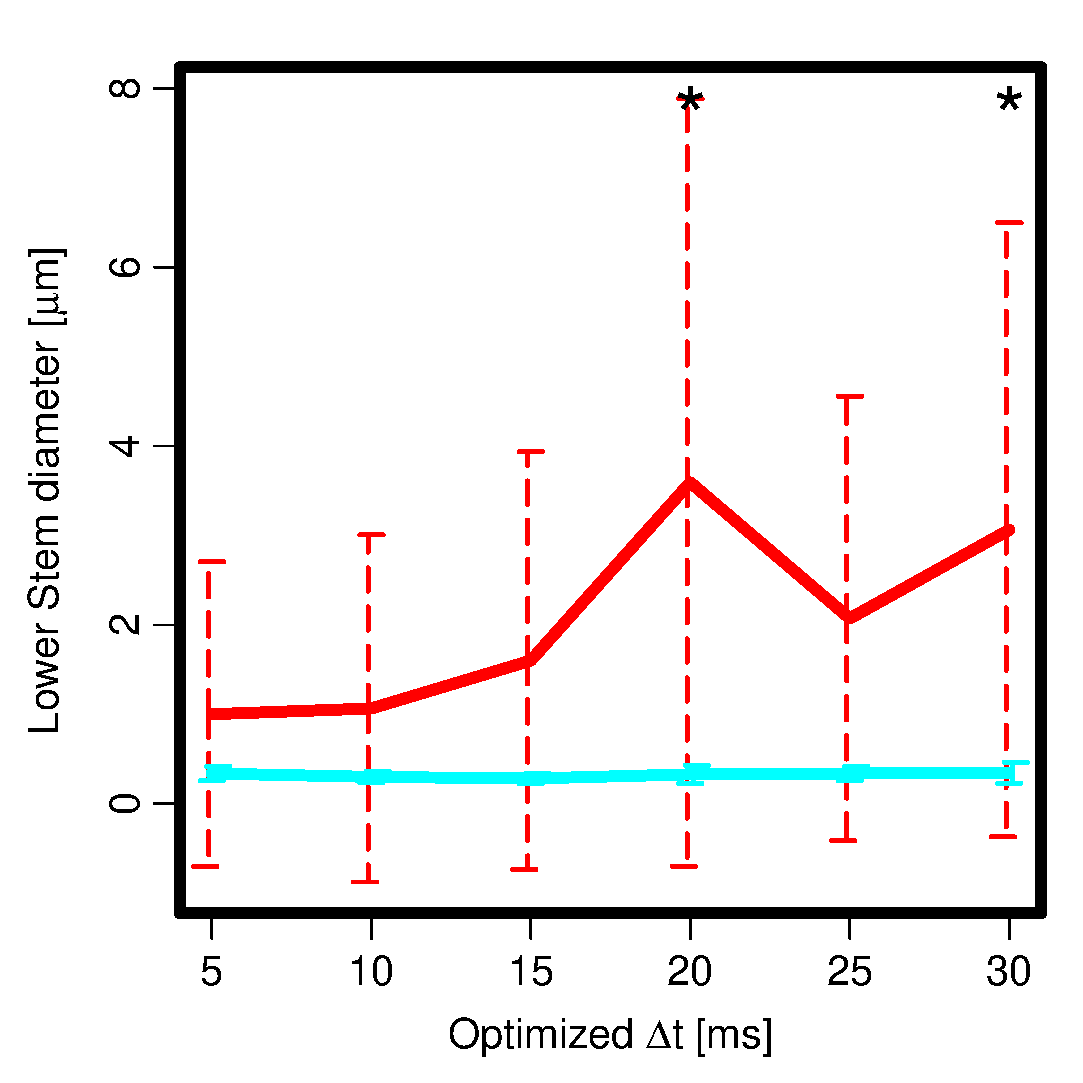
\includegraphics[width=0.8\columnwidth]{./Images_Result/Tsuishi_Rerative_Lower_Diam.eps} 
         \caption{Lower Dendrite$B$ND>7B(B}
         \label{Tsuishi_Rerative_Lower_Diam}
       \end{subfigure}
       %% \begin{subfigure}{0.3\columnwidth}
       %%   \centering
       %%   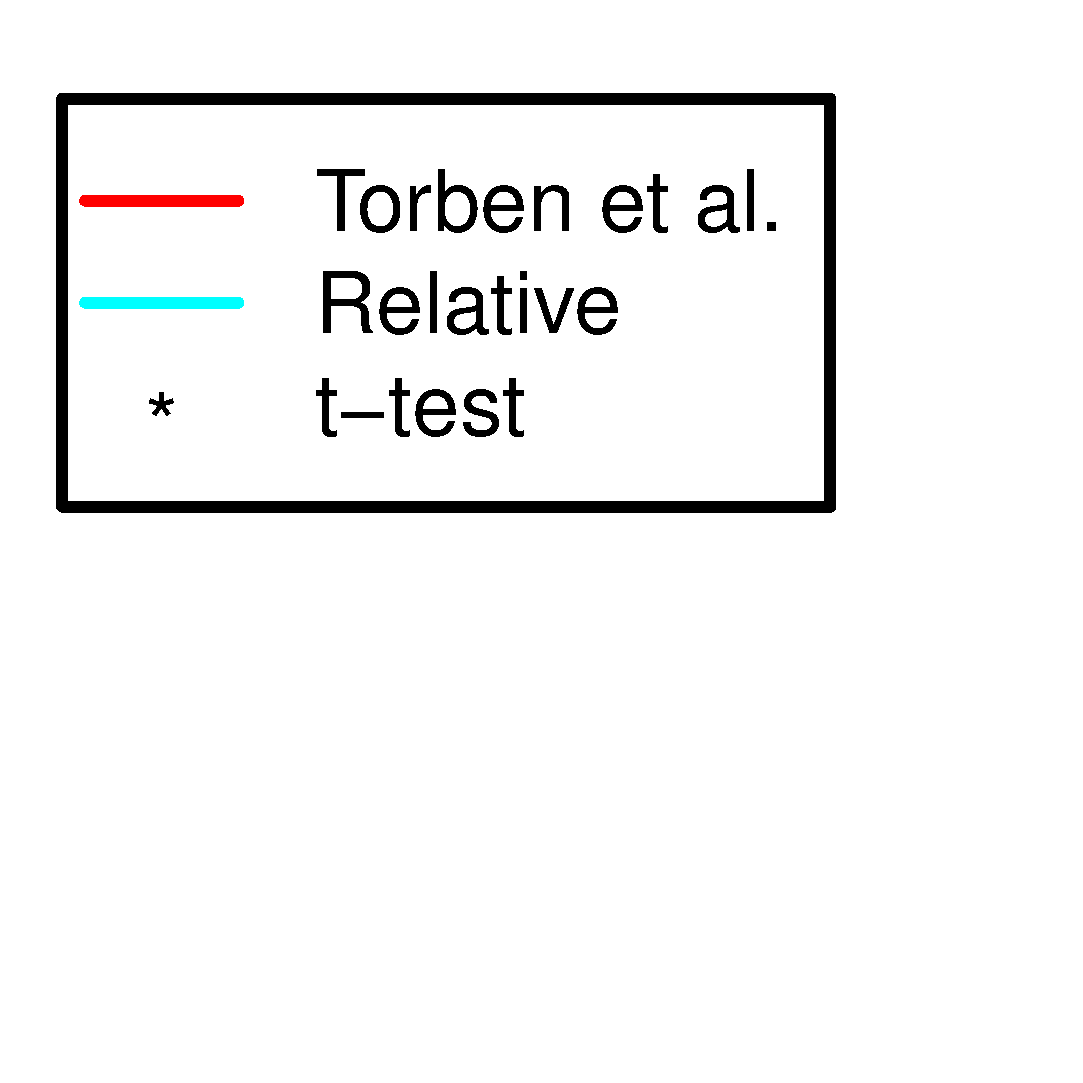
\includegraphics[width=\columnwidth]{./Images_Result/Tsuishi_Rerative_legend.eps} 
       %% \end{subfigure}
       \caption{$B@h9T8&5f<jK!$H$NHf3S(B2}
       \label{Tsuishi_Rerative2}
     \end{figure}

     $B3F(B${\Delta}t$$B$K$*$$$F?^Cf>eIt$N@10u(B(${\star}$)$B$O(B, $B%&%'%k%A$N(Bt$B8!Dj(B(${\alpha} = 0.05$)$B$rMQ$$$F(B 
     $B@h9T8&5f<jK!(B(Torben et al)$B$HK\8&5f<jK!(B(Rerative)$B$NJ?6QCM$rHf3S$7$?:]$K(B, $BM-0Y:9$,$_$i$l$?$3$H$r<($9(B. 
     $B?^(B\ref{Tsuishi_Rerative_F}$B$H?^(B\ref{Tsuishi_Rerative_volume}$B$+$i$o$+$k$h$&$K(B, 2$B$D$N<jK!$N4V$G5!G=@-(B$F$$B$K$O$"$^$j:9$O8+$i$l$J$$$,(B
     $BBN@Q$OL@$i$+$K>.$5$/$J$C$F$$$k(B. 
     $B$^$?(B, 2$B$D$N<jK!(B(${\Delta}t = 15$[ms])$B$G@8@.$5$l$??@7P:YK&$NNc$r?^(B\ref{passive_morphos}$B$K<($9(B. 
%
% $B7ABVNc$O$G$-$?$iJ#?t$N$;$?$$(B, $BGH7A$b$N$;$?$$(B
%
     \begin{figure}[H]
       \begin{subfigure}{0.5\columnwidth}
         \centering
         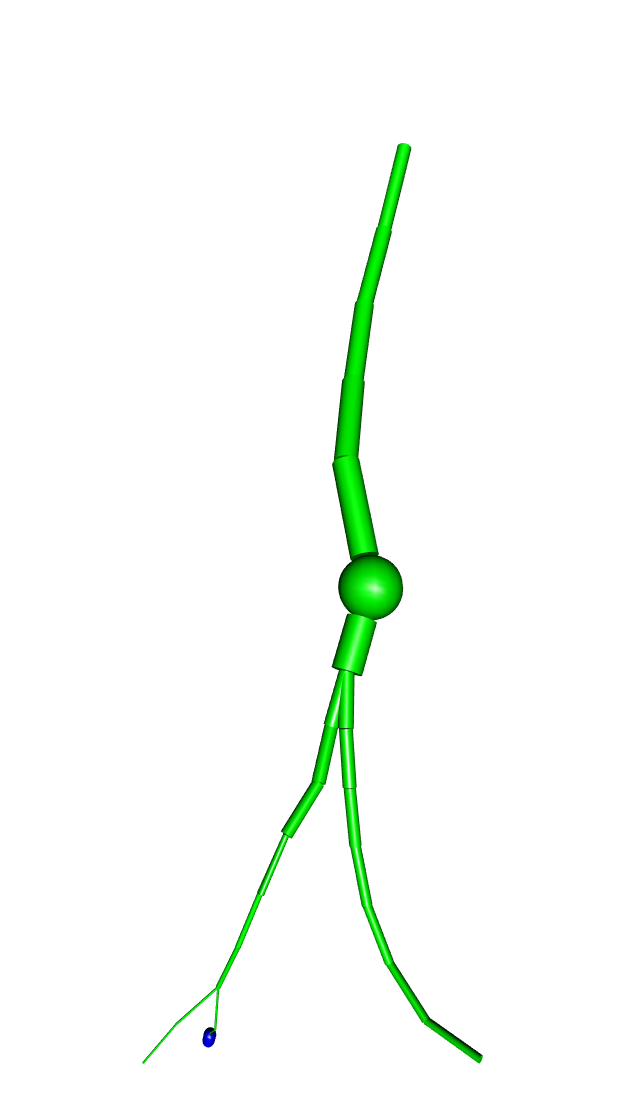
\includegraphics[width=0.7\columnwidth]{./Images_Result/alfa_sample.png} 
         \caption{$B@h9T8&5f<jK!(B}
         \label{Tsuishi_sampel}
       \end{subfigure}
       \begin{subfigure}{0.5\columnwidth}
         \centering
         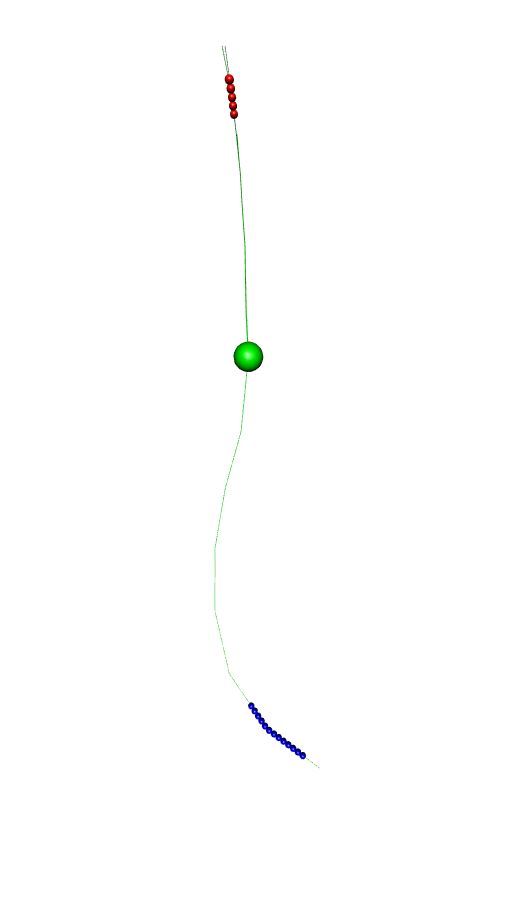
\includegraphics[width=0.5\columnwidth]{./Images_Result/rerative_sample.png}
         \caption{$BK\8&5f<jK!(B}
         \label{Rerative_sampel}
       \end{subfigure}
       \caption{P assive$B?@7P:YK&7A$NBVNc(B}
       \label{passive_morphos}
     \end{figure}

     %
     % $B%7%J%W%90LCV!"D9$5$N%0%i%U$O$b$&>/$72C9)$7$F$+$i=P$7$?J}$,$$$$(B
     %
     %

 \section{Ka$B%A%c%M%k$rMQ$$$?>l9g$N7k2L(B}
   $B?^(B\ref{Ka_Result1}, $B?^(B\ref{Ka_Result2}$B$K(BKa$B%A%c%M%k$rF3F~$7$?:]$N7k2L$r<($9(B. $B?^Cf$N(BGausian$B$O%3%s%@%/%?%s%9J,I[MM<0$K(B
   $B%,%&%9J,I[$rMQ$$$F$*$j(B, Liner$B$O@~7AJ,I[$rMQ$$$?>l9g$N7k2L$G$"$k(B. $B$^$?(B-reduced$B$O$=$l$>$l$N%3%s%@%/%?%s%9J,I[MM<0$G8DBNI>2A$K%3%s%@%/%?%s%9NL$X$N9MN8$rF3F~$7$?>l9g$N7k2L$G$"$k(B.
   $B3F(B${\Delta}t$$B$K$*$$$F(B, Ka$B%3%s%@%/%?%s%9$rF3F~$7$?7k2L(B
   (Gausian, Liner)$B$HA09`$NK\8&5f<jK!(B
   $B$GF@$i$l$?(BPassive$B%b%G%k$N7k2L$r%&%'%k%A$N(Bt$B8!Dj(B($\alpha = 0.05$)$B$rMQ$$$FHf3S$7$?(B.
   Gausian-Passive$B4V$GM-0Y:9$,8+$i$l$?:]$O@V?'$N@10u(B($\star$), Liner-Passive$B4V$K(B
   $BM-0Y:9$,8+$i$l$?:]$K$O@D$$@10u$r?^Cf>eIt$K$D$1$F$$$k(B. $B$^$?(BGausian$B$H(BGausian-reduced,
   Liner$B$H(BLiner-reduced$B$NAH$G$bF1MM$N8!Dj$r9T$$(B, $BM-0U:9$,$_$i$l$?:]$K$O$=$l$>$l(B
   $B\t?'(B, $B?e?'$N==;z$r5-:\$7$F$$$k(B.

   % Gausian$B$H(B-reduced$B$rHf$Y$k$J$iJRB&8!Dj$N$[$&$,$h$/$J$$$+!)(B
   %
   % $B8!Dj7k2L$,J#;($J$N$GI=$K$7$?$[$&$,$$$$$+$b(B
   % $B$G$b@~7AJ,I[$,%,%&%9J,I[$h$j$b$h$$<gD%$9$k$3$H$K0UL#$O$"$k$+!)(B
   %
   
     \begin{figure}[H]
       \begin{subfigure}{0.5\columnwidth}
         \centering
         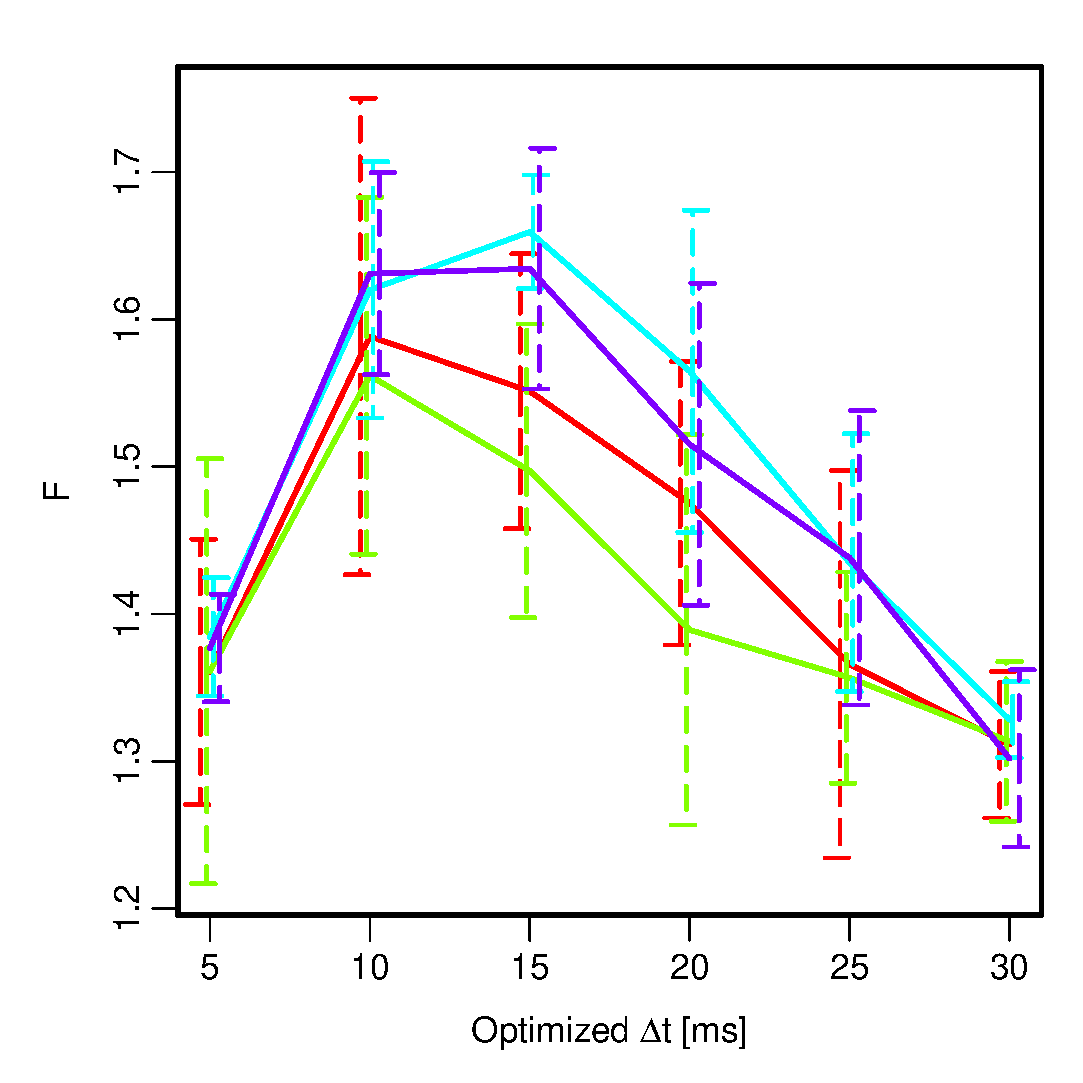
\includegraphics[width=0.8\columnwidth]{./Images_Result/k_test_F.eps}
         \caption{F}
         \label{k_F}
       \end{subfigure}
       \begin{subfigure}{0.5\columnwidth}
         \centering
         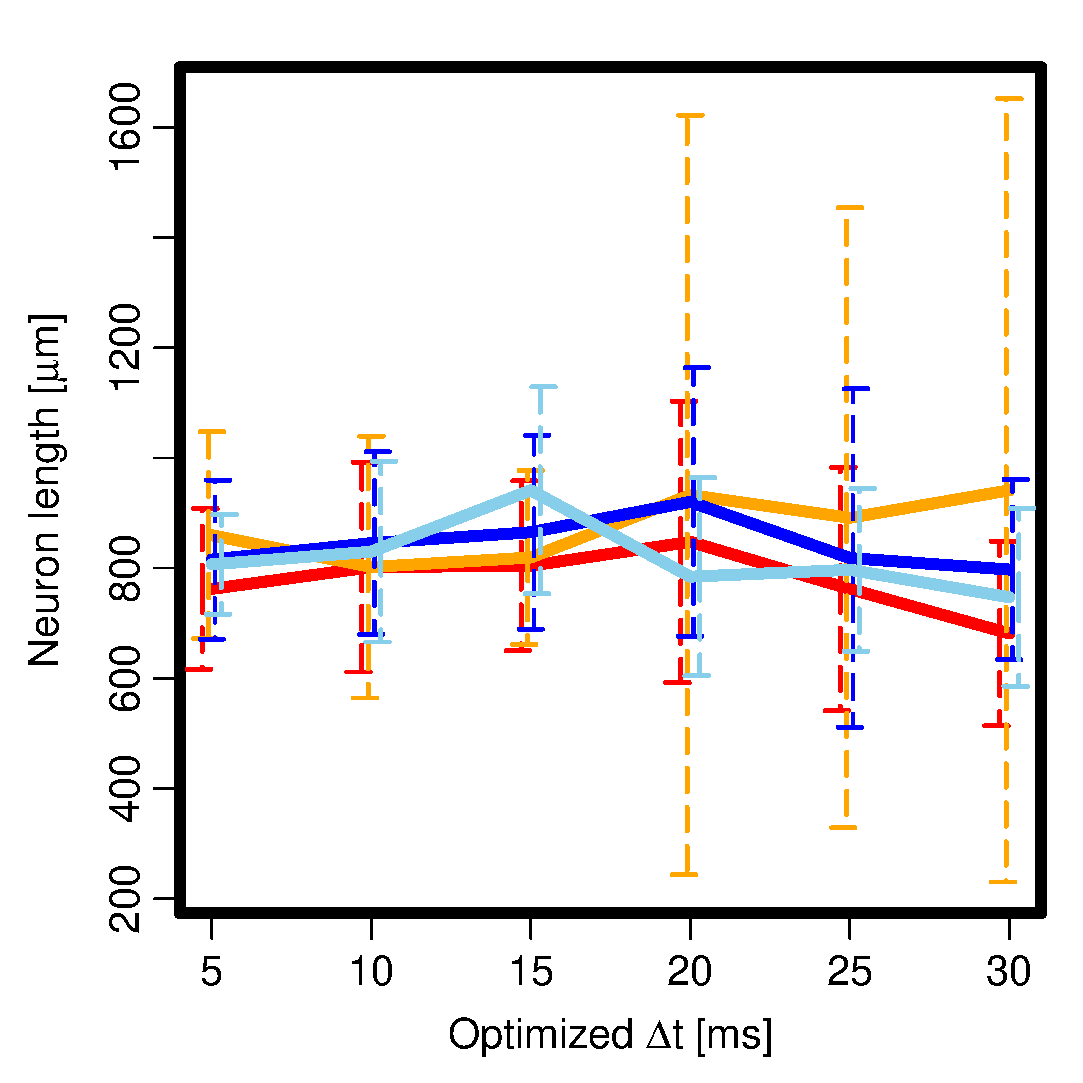
\includegraphics[width=0.8\columnwidth]{./Images_Result/k_test_TREE_length.eps} 
         \caption{$BD9$5(B}
         \label{k_TREE_length}
       \end{subfigure}

       \begin{subfigure}{0.5\columnwidth}
         \centering
         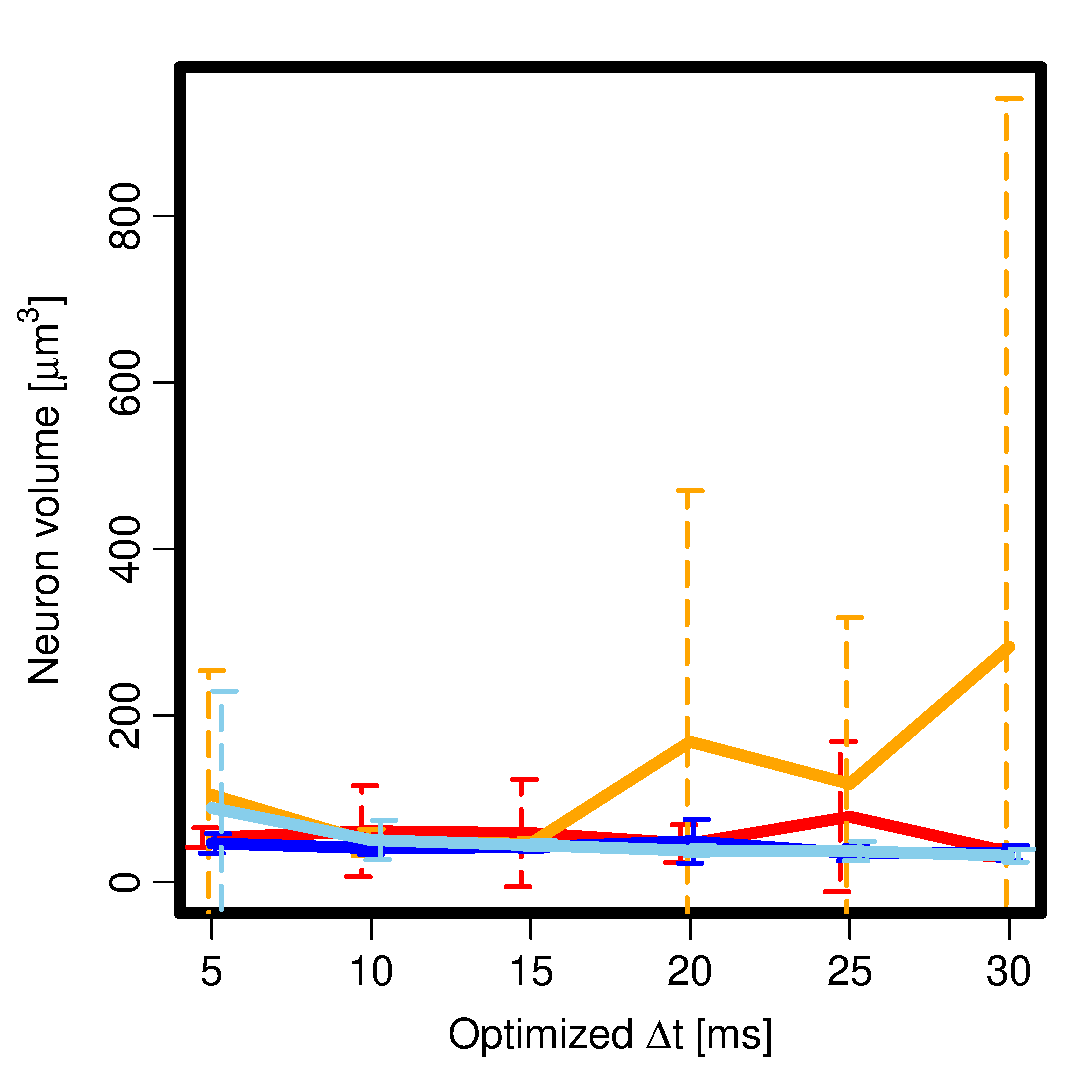
\includegraphics[width=0.8\columnwidth]{./Images_Result/k_test_TREE_volume.eps}
         \caption{$BBN@Q(B}
         \label{k_TREE_volume}
       \end{subfigure}
       \begin{subfigure}{0.5\columnwidth}
         \centering
         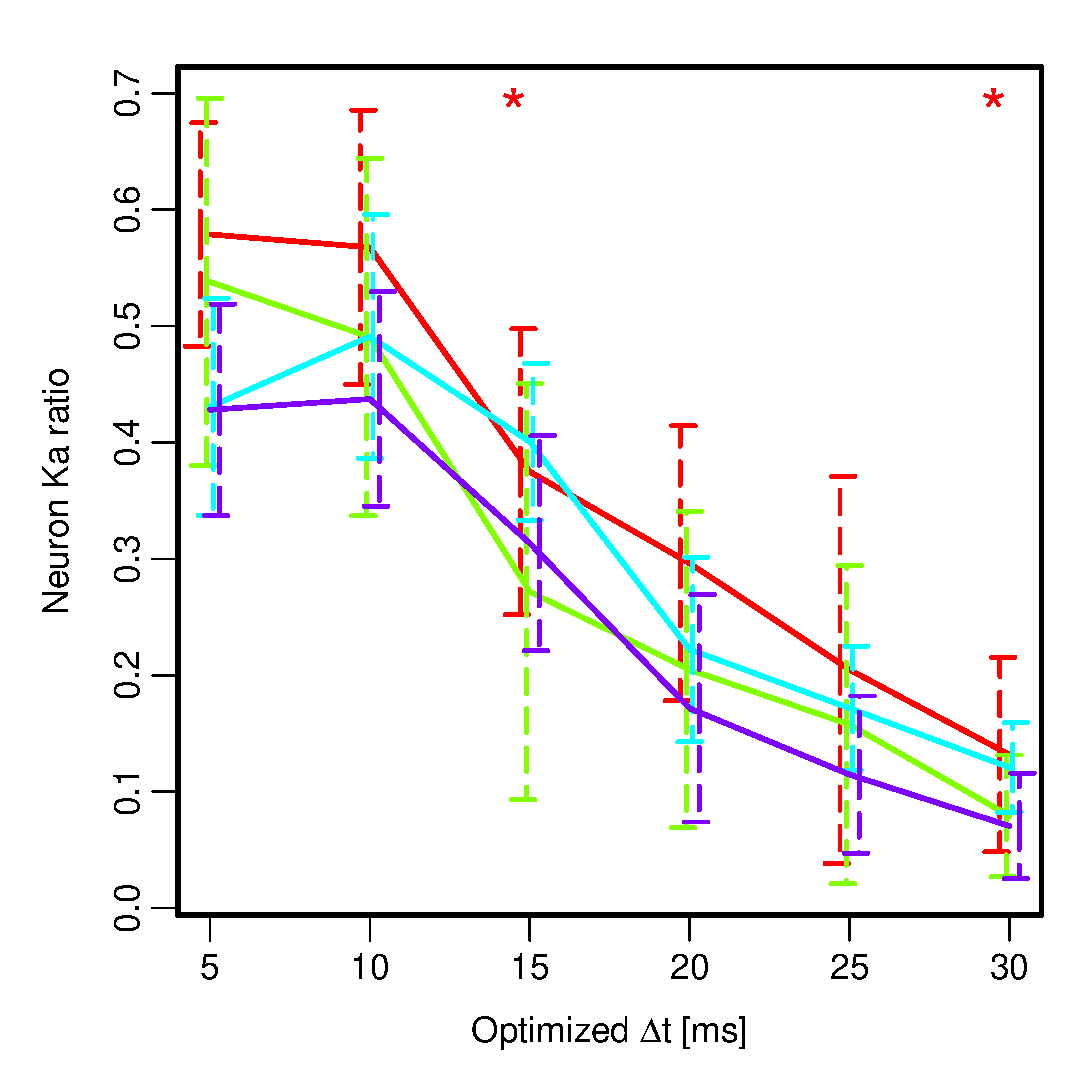
\includegraphics[width=0.8\columnwidth]{./Images_Result/k_test_TREE_K_ratio.eps}
         \caption{Ka$B%3%s%@%/%?%s%94^M-N((B}
         \label{k_TREE_K_ratio}
       \end{subfigure}

       \begin{subfigure}{\columnwidth}
         \centering
         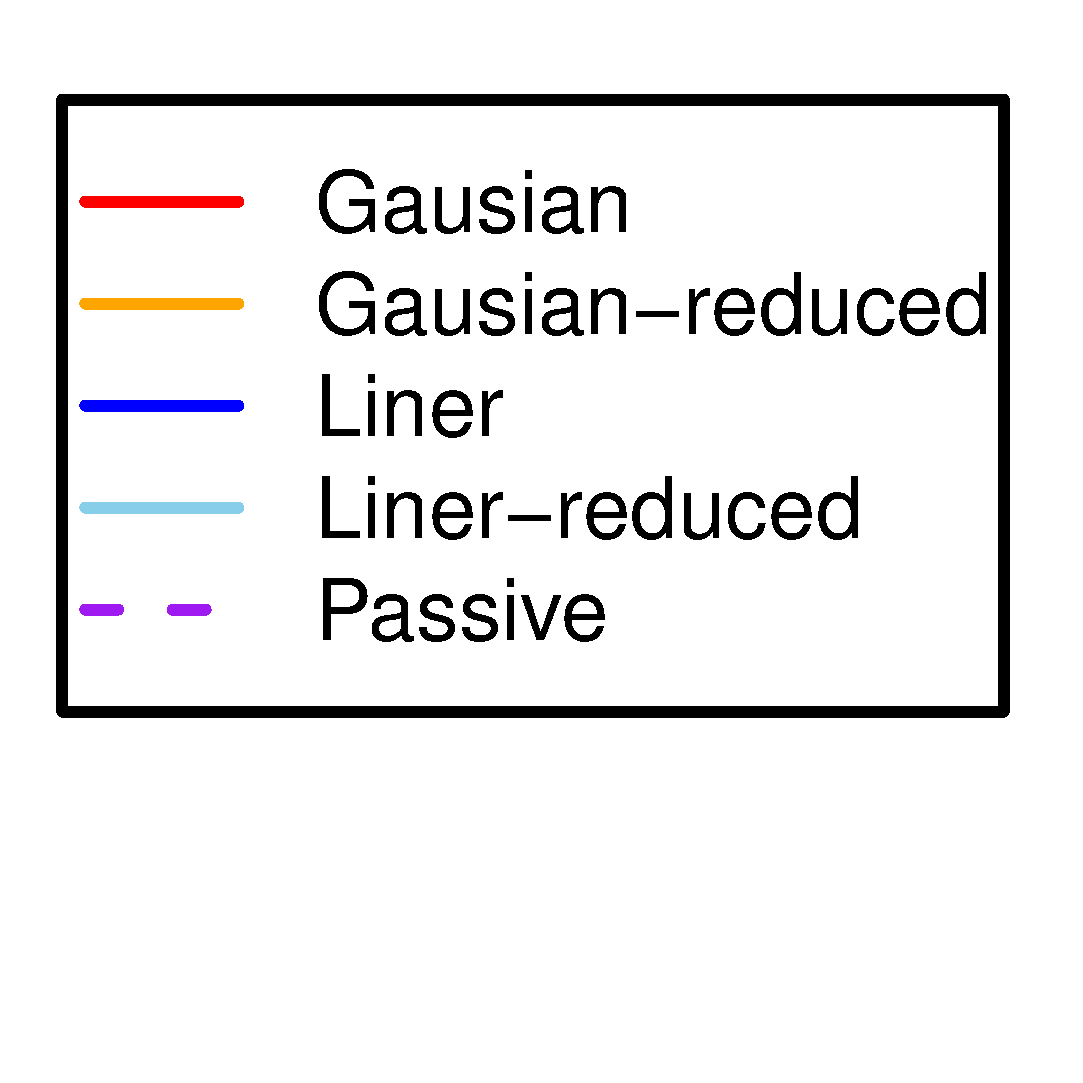
\includegraphics[width=0.3\columnwidth]{./Images_Result/k_test_legend.eps} 
       \end{subfigure}

       \vspace{-3cm}
       \caption{Ka$B%A%c%M%k$rF3F~$7$?:]$N7k2L(B1} %$B%Z!<%8%l%$%"%&%H$,7hDj$7$F$+$iHyD4@0$9$k(B
       \label{Ka_Result1}
     \end{figure}

     \begin{figure}[H]
       \begin{subfigure}{0.5\columnwidth}
         \centering
         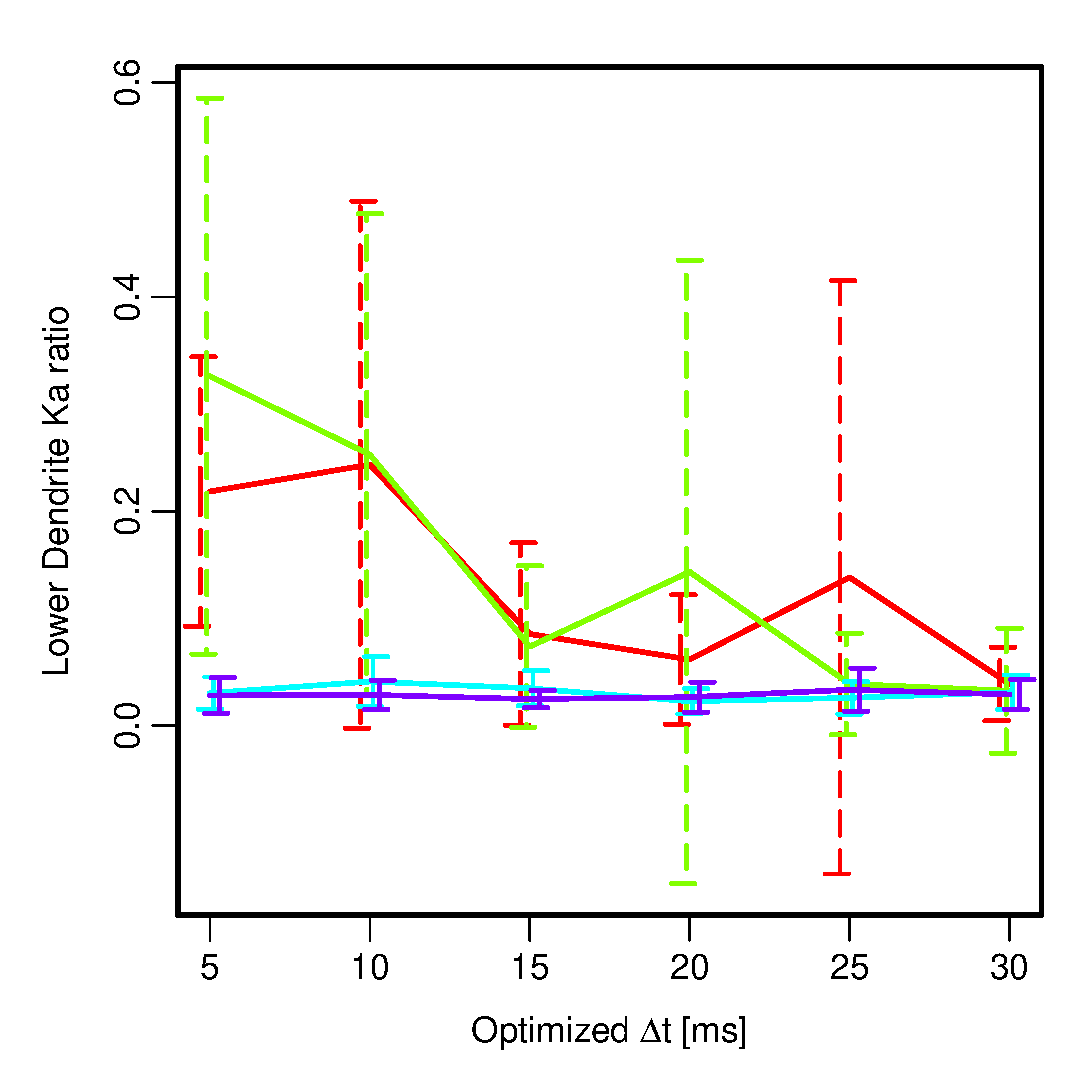
\includegraphics[width=0.8\columnwidth]{./Images_Result/k_test_Lower_K_ratio.eps}
         \caption{Lower Dendrite$B$N(BKa$B%3%s%@%/%?%s%94^M-N((B}
         \label{k_lower_ratio}
       \end{subfigure}
       \begin{subfigure}{0.5\columnwidth}
         \centering
         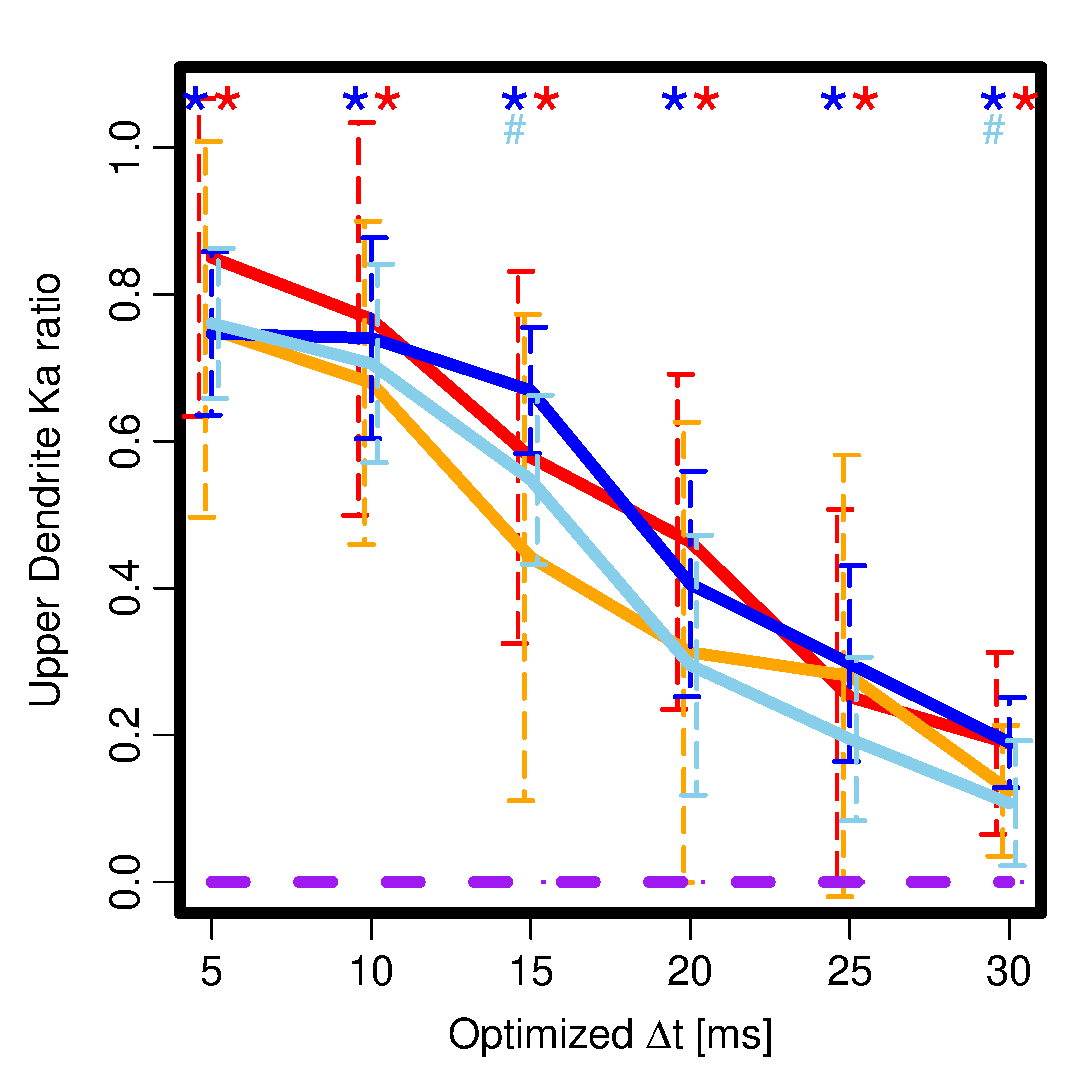
\includegraphics[width=0.8\columnwidth]{./Images_Result/k_test_Upper_K_ratio.eps}
         \caption{Upper Dendrite$B$N(BKa$B%3%s%@%/%?%s%94^M-N((B}
         \label{k_upper_ratio}
       \end{subfigure}

       \begin{subfigure}{\columnwidth}
         \centering
         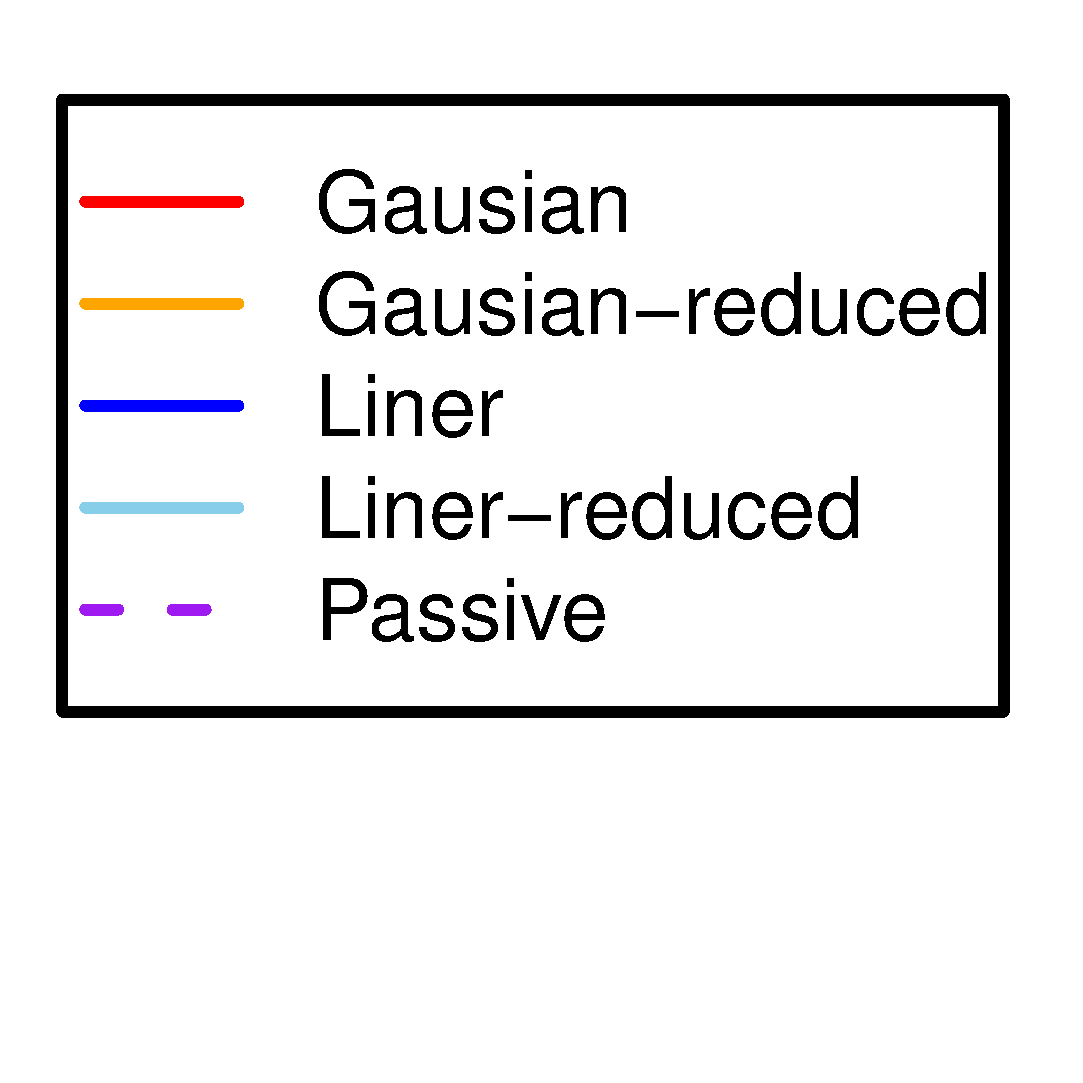
\includegraphics[width=0.35\columnwidth]{./Images_Result/k_test_legend.eps} 
       \end{subfigure}
       \vspace{-1.9cm}
       \caption{Ka$B%A%c%M%k$rF3F~$7$?:]$N7k2L(B2} %$B%Z!<%8%l%$%"%&%H$,7hDj$7$F$+$iHyD4@0$9$k(B
       \label{Ka_Result2}
     \end{figure}

     \begin{figure}[H]
       \begin{subfigure}{\columnwidth}
         \centering
         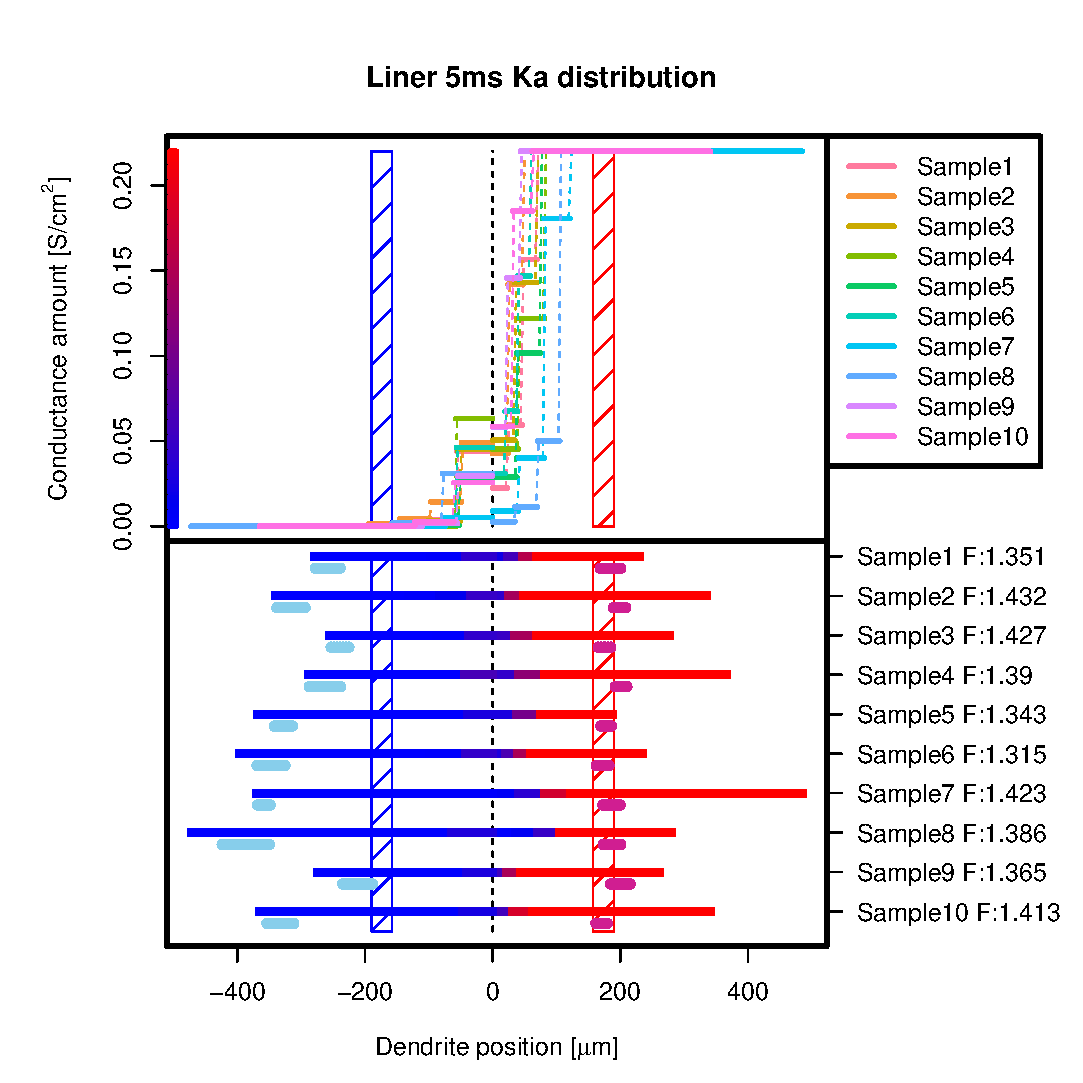
\includegraphics[width=0.75\columnwidth]{./Images_Result/k_Rerative_liner_75_0_K_distribution_dt5.eps}
         \caption{}
         \label{k_lower_ratio}
       \end{subfigure}

       \begin{subfigure}{\columnwidth}
         \centering
         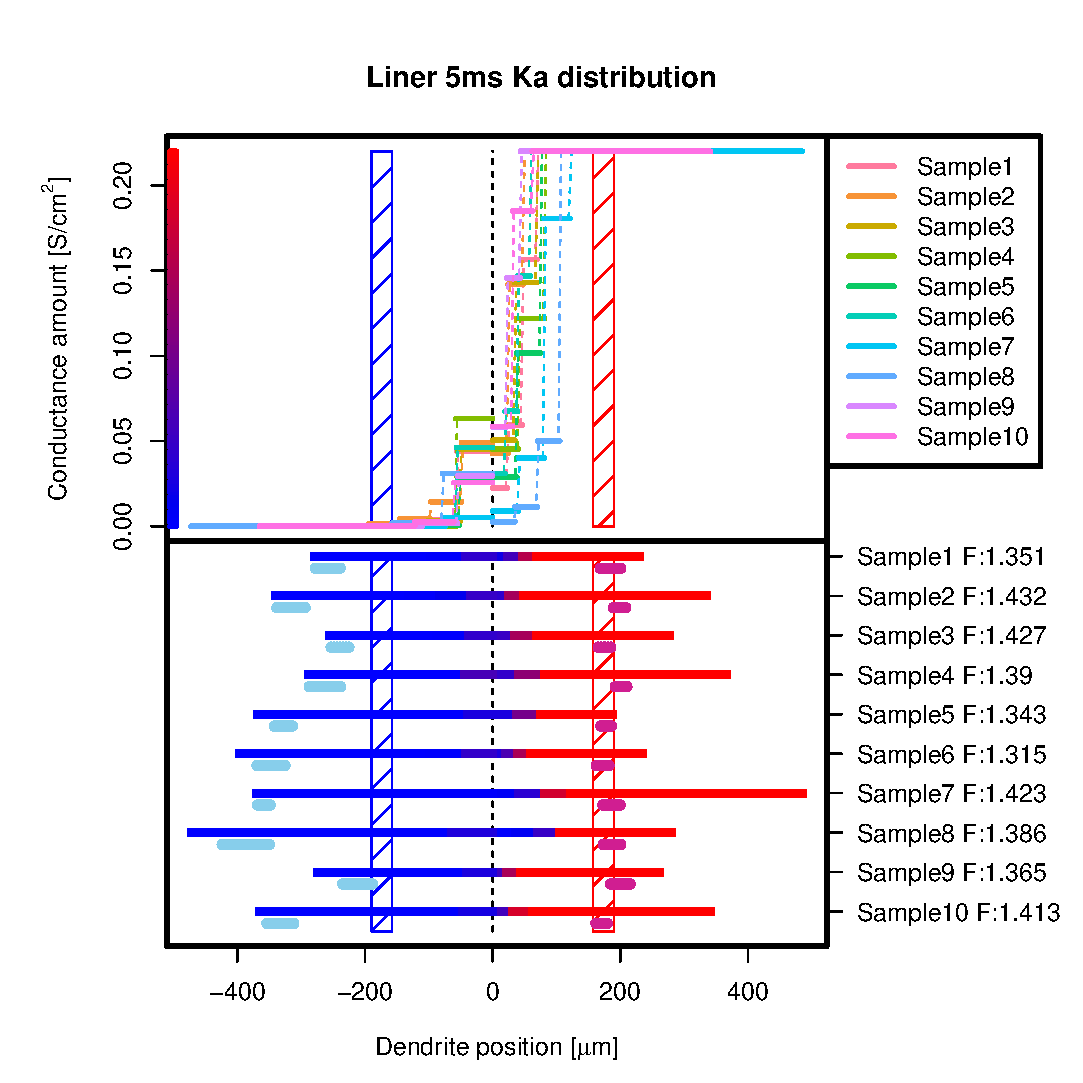
\includegraphics[width=0.75\columnwidth]{./Images_Result/k_Rerative_liner_75_0_K_distribution_dt5.eps}
         \caption{Lower Dendrite$B$N(BKa$B%3%s%@%/%?%s%94^M-N((B}
         \label{k_lower_ratio}
       \end{subfigure}

       \caption{${\Delta}t = 5$[ms]$B$G$N(BKa$B%3%s%@%/%?%s%9J,I[(B}
       \label{Ka_Result3}
     \end{figure}
 
 \section{CaT$B%A%c%M%k$rMQ$$$?>l9g$N7k2L(B}

 \section{Ka$B%A%c%M%k(B, CaT$B%A%c%M%k$rMQ$$$?>l9g$N7k2L(B}

% $B:G8e$K$=$l$>$l$NJ,I[%Q%?!<%s!"%3%s%@%/%?%s%99MN8$NAH$G!"(B4$B%Q%?!<%s$N%3%s%@%/%?%s%9$K$h$k7k2L$r0l$D$N%0%i%U$K$^$H$a$k(B
